\chapter{Theoretische Grundlagen}

\section{Begriffsdefinitionen}
In den folgenden Kapiteln werden die Begriffe ``Social Network Analysis'', ``Social Forces'', ``Graph'' und ``Link Prediction'' einzeln
erläutert. Es handelt sich in Bezug auf die Arbeit um grundlegende Begriffe. Weitere Fachbegriffe, die
in der Arbeit verwendet werden, sind im Glossar beschrieben.

\subsection{Social Network Analysis}
Soziale Netzwerke bestehen aus Akteuren, wie beispielsweise Individuen, Organisationen oder ganze Nationen und deren Beziehungen (\citeauthor{ulrike_baumol_soziale_2019} \citeyear{ulrike_baumol_soziale_2019}, online).
Unter \acl{sna} (SNA, dt. Soziale Netzwerkanalyse) wird die Methode zur Erfassung und Analyse dieser Netzwerke und der Beziehungen darin verstanden (\citeauthor{wikipedia_soziale_2019} \citeyear{wikipedia_soziale_2019}, online).
Die soziale Netzwerkanalyse ist ein interdisziplinäres Forschungsfeld und wird nach \cite{ulrike_baumol_soziale_2019} in den Sozial- und Verhaltenswissenschaften aber auch in der Betriebswirtschaftslehre oder den Politikwissenschaften angewandt.
Gegenwärtig sind sogenannte ``soziale Netzwerke'' allgegenwärtig und werden insbesondere im Kontext von Internet-Plattformen wie \textit{Facebook} oder \textit{Twitter} häufig betrachtet.

\subsection{Social Forces}
\label{socialforces}
In sozialen Netzwerken wird die Wahrscheinlichkeit für das Entstehen und Erhalten von Kanten durch unterschiedliche
Faktoren begünstigt. Dazu gehören die Social Forces, die man in sechs Hauptkategorien unterteilen kann: Homophilie,
Reziprozität, Nähe, Ansehen, soziale Anpassung und Transivität. Im folgenden Abschnitt werden diese Kategorien kurz
beschrieben. Für die in dieser Arbeit implementierten Algorithmen sind dabei vor allem Transitivität und Ansehen
relevant.

\subsubsection{Homophilie}
Homophilie beruht darauf, dass zwei Knoten, die Gemeinsamkeiten aufweisen, eine höhere Wahrscheinlichkeit dafür
aufweisen, eine Verbindung aufzubauen. Hier sind beispielsweise Hobbys oder die politische Orientierung relevant. Wollte
man für diese Art der sozialen Kräfte einen Algorithmus zur Link Prediction entwerfen, müsste dieser vorhandene
Attribute miteinander vergleichen, beispielsweise das Attribut "Lieblingsband". Stimmt die Band in diesem Attribut
überein, wäre dann laut dem Prinzip der Homophilie die Wahrscheinlichkeit höher, dass eine neue Kante entsteht.

\subsubsection{Reziprozität}
Reziprozität oder einfacher formuliert "Gegenseitigkeit" bedeutet, dass man eher mit einer Person Kontakt hat, wenn
diese mit einem Kontakt aufnimmt. Wenn A also B eine Nachricht schreibt, erhöht dies die Wahrscheinlichkeit, dass B auf
die Nachricht reagiert und A antwortet - eine Ausnahme stellen hier zum Beispiel prominente Personen dar.

Diese Art der Social Forces wäre also vor allem in gerichteten Graphen relevant, da in ungerichteten Graphen die
Richtung der Kanten nicht bestimmt ist. Eine Vorhersage zur Entstehung neuer Kanten müsste dabei dann aber auch über
andere Social Forces geschehen, um den initialen Kontakt, bei dem A sich an B wendet, vorherzusagen.

\subsubsection{Nähe}
Der Begriff Nähe kann in zwei Unterkategorien unterteilt werden. Hierbei geht es um "organisatorische" und
"physikalische Nähe".

Die organisatorische Nähe kommt durch Zusammenarbeit zustande, auch wenn man sich eventuell nicht
am selben Ort befindet. Durch die Angehörigkeit derselben Abteilung in einer Firma steigt jedoch die Wahrscheinlichkeit
für eine Interaktion und somit für die Bildung einer Kante. Diese Art der sozialen Kraft könnte also beispielsweise
über Attribute wie "Abteilung" oder "Firma" überprüft werden. In der Umsetzung eines Algorithmus wäre diese Art der
Nähe also sehr ähnlich wie die der Homophilie.

Die physikalische Nähe bezieht sich hingegen direkt darauf, wie oft man eine Person sieht. Ist man häufiger in
unmittelbarer Nähe einer Person, bevorzugt man diese tendentiell. Für die Bestimmung dieses Wertes muss also ein Attribut
gefunden werden, mit welchem sich die Distanz bestimmen lässt. Als Beispiel könnte man hier zwei Studenten nehmen,
welche die gleiche Klasse besuchen und beide häufig anwesend sind. Die Wahrscheinlichkeit ist höher, dass sich die
physikalische Nähe positiver auf ihre Beziehung zueinander auswirkt, als bei zwei Studenten, bei denen nur einer oder
beide selten den Unterricht besuchen.

\subsubsection{Ansehen}
Das Ansehen wird hauptsächlich über die Vernetzung einer Person definiert. Bei der Vernetzung ist es von Vorteil, wenn
man die Normen und Werte einer Gruppe teilt und fördert. Dies erleichtert es, Zugang zu mehr Personen zu erhalten. Es
kann ausserdem auch sein, dass man sich gruppenübergreifend vernetzt. In diesem Fall kann es zu Konflikten kommen, wenn
verschiedene Werte vertreten werden. Als Beispiel kann man Musiker nennen, die ihre politische Meinung äussern. Sie
haben zuvor einen Fankreis aufgebaut, der aus verschiedenen Gruppen besteht, die unterschiedliche Werte und Normen
haben können. Äussert der Musiker nun zum ersten Mal eine politische Meinung, kann dies in einigen der Gruppen auf
Zuneigung, in anderen auf Ablehnung stossen. Aus diesem Grund wird es auch solche Personen geben, die Meinungen, die
nicht den Gruppennormen und -werten entsprechen, geheimhalten, um besser in die Gruppe zu passen.

Ein Algorithmus für die Vorhersage von neuen Kanten könnte beim Ansehen ähnlich aussehen wie bei der Homophilie und über
Gemeinsamkeiten neue Kontakte ausmachen - oder aber er bezieht die Vernetzung im allgemeinen ein, in dem man die Frage
stellt, wie beliebt zwei Personen bereits im Netzwerk sind. Je beliebter, desto höher die Wahrscheinlichkeit einer
möglichen Vernetzung.

\subsubsection{Soziale Anpassung}
Die soziale Anpassung fliesst etwas in das Thema Ansehen hinein. Auch hier geht es um Gruppennormen und -werte. Hierbei
geht es aber explizit, um die Anpassung der Meinung in Bezug auf die Zugehörigkeit einer Gruppe. Hier geht es weniger
um die Vernetzung untereinander, sondern um die Auswirkungen eben jener Vernetzung.

Analysieren könnte man eine solche soziale Anpassungen zum Beispiel, indem man Netzwerke über längere Zeiträume
beobachtet. Wird hier beispielsweise Person A in eine Gruppe integriert und ändert daraufhin eines ihrer Merkmale,
beispielsweise die politische Ausrichtung, und steht dies im Einklang mit der Gruppe, ist es wahrscheinlich, dass dies
aufgrund des sozialen Drucks geschehen ist. Dies wird wahrscheinlich, wenn A mit Person B, welche ein hohes Ansehen in
der Gruppe geniesst, direkt vernetzt ist, da B einen sehr grossen Einfluss hat.

\subsubsection{Transitivität}
Transitivität ist sehr ähnlich zur Homophilie. Hier geht es allerdings nicht darum, ob man gemeinsame Eigenschaften,
soondern ob man gemeinsame Freunde vorzuweisen hat. Die Wahrscheinlichkeit, dass A, der mit B befreundet ist, irgendwann
auf C trifft - ein Freund von B -, und dass A und C sich verstehen, ist höher als sich mit einer zufälligen Person auf
der Strasse anzufreunden. Hier spielen sicherlich auch andere Kräfte wie das Ansehen und die Nähe eine Rolle.

\subsection{Graph}
Soziale Netzwerke können einfach als Graph modelliert werden.
Ein Graph $G = (V, E)$ besteht aus einer Menge $V = \{1,2,...,|V|\}$ von Knoten und Kanten $E \subseteq V\times V $ (vgl. \citeauthor{ottmann_algorithmen_2017} \citeyear{ottmann_algorithmen_2017}, S. 590).
Die Knoten repräsentieren dabei Akteure, während die Kanten die Beziehungen zwischen den Akteuren repräsentieren.
Abbildung \ref{fig:graph_undirected} zeigt einen ungerichteten Graphen. Die Kanten enthalten dabei keine Pfeile, was verdeutlicht, dass die Interaktion in beide Richtungen erfolgen kann.
Ein Beispiel für einen ungerichteten Graphen ist das Freundes-Netzwerk von \textit{Facebook}.

\begin{figure}[h]
    \centering
    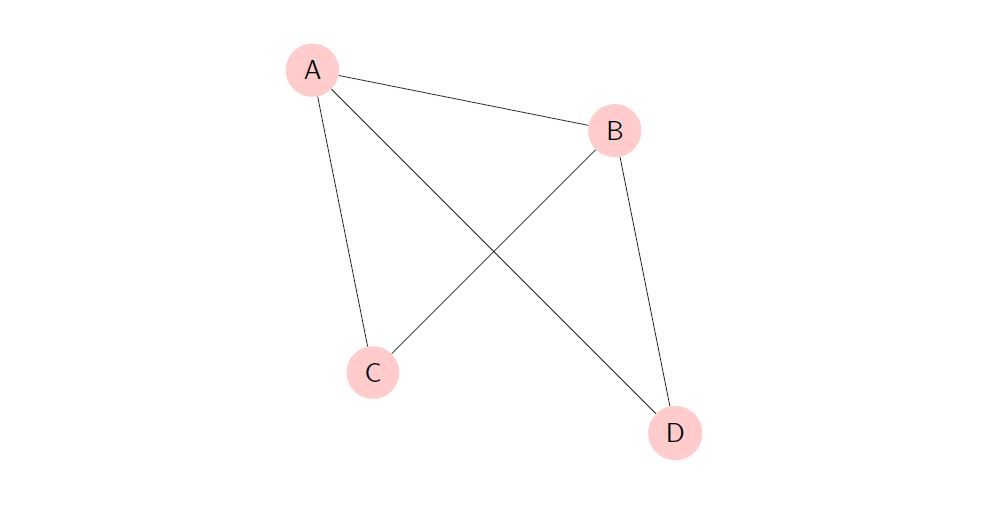
\includegraphics[scale=0.7]{resources/graph_undirected.JPG}
    \caption{Ungerichteter Graph}
    % TODO Add cite to SNA Script
    \label{fig:graph_undirected}
\end{figure}

Im Gegensatz dazu gibt es bei einem gerichteten Graphen eine Quelle und ein Ziel. Die Richtung der Interaktion wird durch einen Pfeil visualisiert.
Abbildung \ref{fig:graph_directed} zeigt einen solchen Graphen.
Als Beispiel für einen gerichteten Graphen dient ein E-Mail Netzwerk. Jede Nachricht wird dabei von einem Sender an einen Empfänger versendet.

\begin{figure}[h]
    \centering
    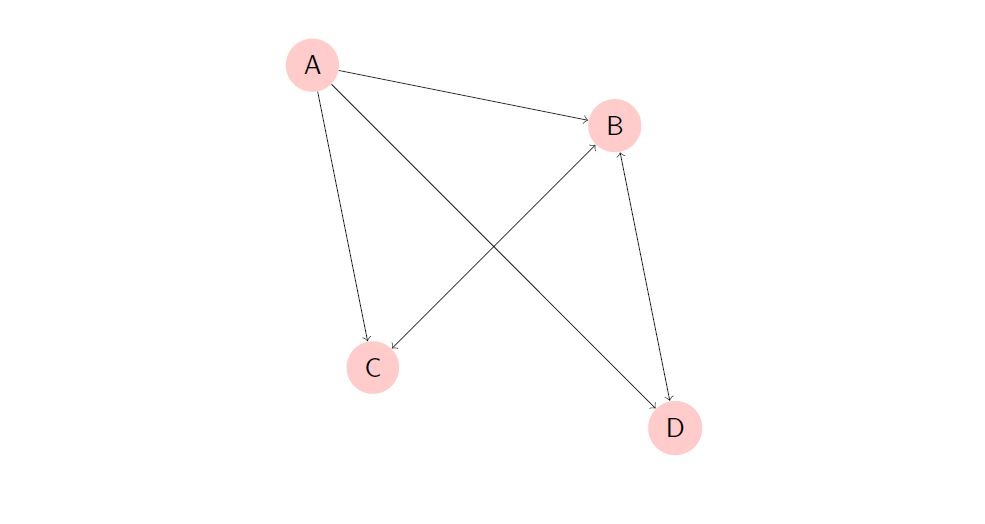
\includegraphics[scale=0.7]{resources/graph_directed.JPG}
    \caption{Gerichteter Graph}
    % TODO Add cite to SNA Script
    \label{fig:graph_directed}
\end{figure}

\subsection{Link Prediction}
Link Prediction baut auf einem bestehenden Netzwerk auf und versucht vorherzusagen, welche Kanten sich als nächstes bilden werden:
Der Graph $G = (V, E)$, bestehend aus Knoten ($V$, engl. Vertices) und Kanten ($E$, engl. Edges), hat sich in einem Zeitintervall $G[t, t_1]$ gebildet.
In einem nächsten Zeitintervall $G[t_1, t_2]$ könnten neue Kanten zum Netzwerk hinzukommen.
Mittels Link Prediction wird nun versucht vorherzusagen, welche Kanten in welcher Reihenfolge zum Graphen hinzugefügt werden (\citeauthor{gao_link_2015} \citeyear{gao_link_2015}, S. 4).
Für solche Vorhersagen gibt es verschiedene Algorithmen mit unterschiedlichen Charakteristiken.
Je nach Eigenschaften des vorliegenden Netzwerks und allfälliger Kontextinformationen liefert ein Algorithmus bessere oder schlechtere Resultate.
Pro Anwendungsfall muss deshalb evaluiert werden, welcher Algorithmus sich am besten eignet.
Der Aufbau der dazu benötigten Messwerte und die daraus folgende Evaluation wird im Kapitel \ref{daten} beschrieben.
